%!TEX root = ../report.tex
\section{Pitchfork}


The cheapest way to continue on the stable, non-symmetric branch of the pitchfork is to break the symmetry of the PDE temporarily. This is carried out by adding a non-symmetric forcing term to the equation controlled by a new parameter {\tt asym}, continuing only a tad in the new parameter, subsequently continuing in $Re$ past the pitchfork bifurcation point, and lastly restoring symmetry by bringing {\tt asym} back to 0. To be more precise, we replace the wind stress forcing term $\tau_x$ by
\begin{equation}
    \tau_x := -\eta \left( \frac{1 - \mathtt{asym}}{2 \pi} \cos(2\pi y) + \frac{\mathtt{asym}}{\pi} \cos(\pi y) \right)
\end{equation}
such that the corresponding term in the right-hand side of the PDE~\eqref{eq:pde} becomes
\begin{equation}
    -\frac{\partial \tau_x}{\partial y} = -\eta (1 - \mathtt{asym})\sin(2\pi y) + \mathtt{asym}\sin(\pi y)).
\end{equation}
This clearly breaks the anti-symmetry $\partial_y \tau_x(y) \neq -\partial_y \tau_x(1 - y).$ We add the parameter $\mathtt{asym}$ at $Re = 16$ and continue in $\mathtt{asym}$ for two steps of $\Delta s = 0.1.$ We then continue in $Re$ until $Re \approx 31.$ At this point it becomes clear we have passed the pitchfork bifurcation point, by judging the behaviour of the solution as shown in Figure~\ref{fig:pitch_detection}. If we look at $\psi_{max}$ as a function of $Re,$ we see interesting behaviour around $Re \approx 29,$ where it suddenly increases and then flattens. Also the effective step size in $Re$ decreases while $\Delta s$ is kept constant at $0.1$; this could mean that the solution changes more rapidly. Even more pronounced is the graph of $\psi_{max} + \psi_{min}$ where we not only see the small disturbance in symmetry around $Re = 16,$ but as well how it blows up past $Re = 29.$ Another way to detect the bifurcation point is to look at a specific point of the solution such as $\psi(\tfrac{1}{8}, \tfrac{1}{8})$ or $\psi(\tfrac{3}{8}, \tfrac{3}{8})$ where a qualitative change in behaviour appears after $Re = 29.$

At $Re \approx 31$, we bring back $\texttt{asym}$ to $0.$ Next we continue to $Re = 40$ at which point we obtain the solution as plotted in Figure~\ref{fig:question_e}.

\begin{figure}[h!]
    \centering
    \caption{Detection of the pitchfork.}
    \label{fig:pitch_detection}
    \centerline{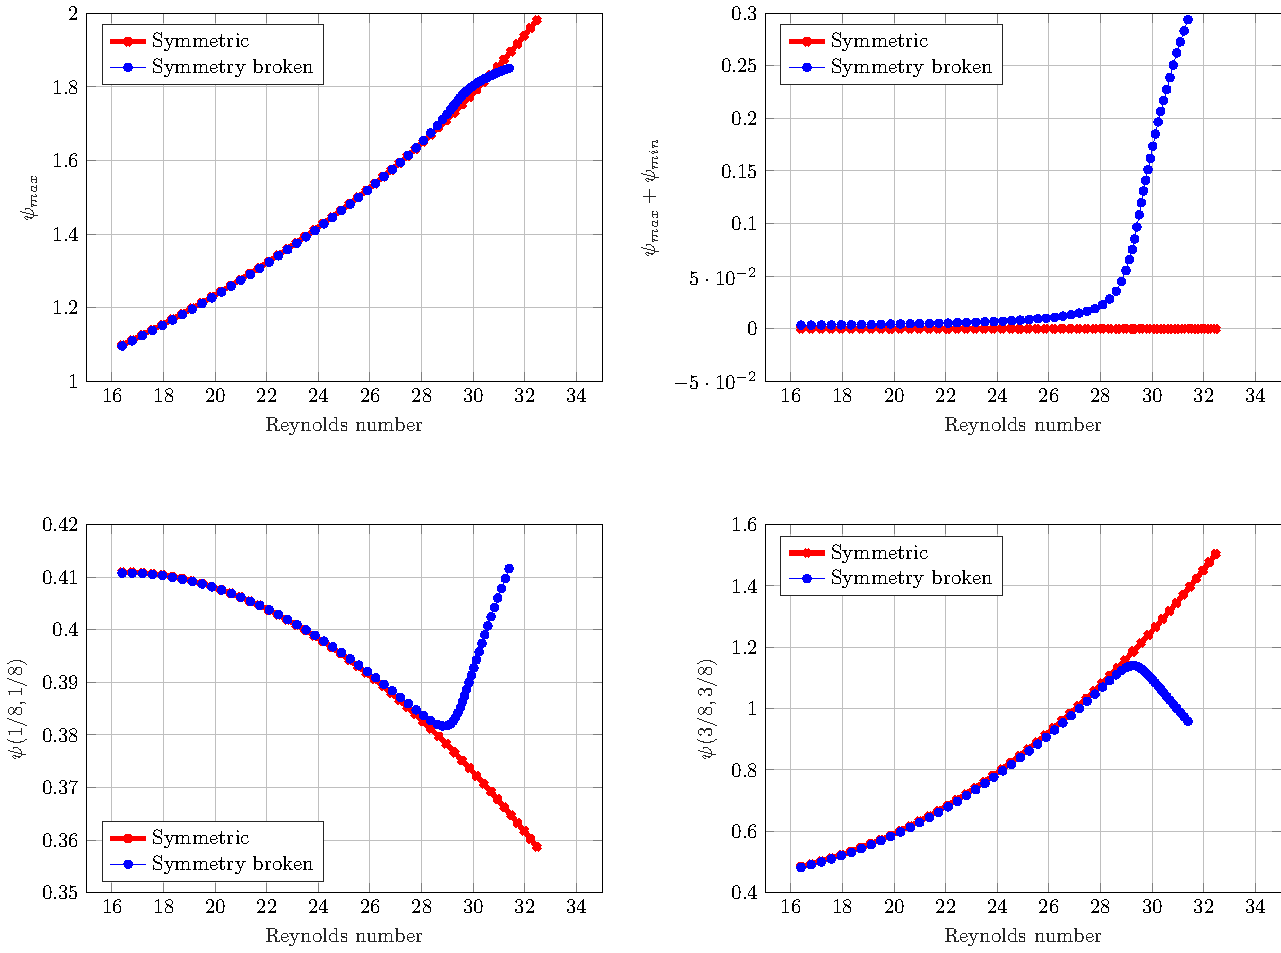
\includegraphics[width=1\textwidth]{images/pitch_detection.pdf}}
\end{figure}

\begin{figure}[h]
    \centering
    \caption{Solutions on the upper branch of the pitchfork}\label{fig:question_e}
    \centerline{
    \begin{subfigure}[b]{0.6\textwidth}
        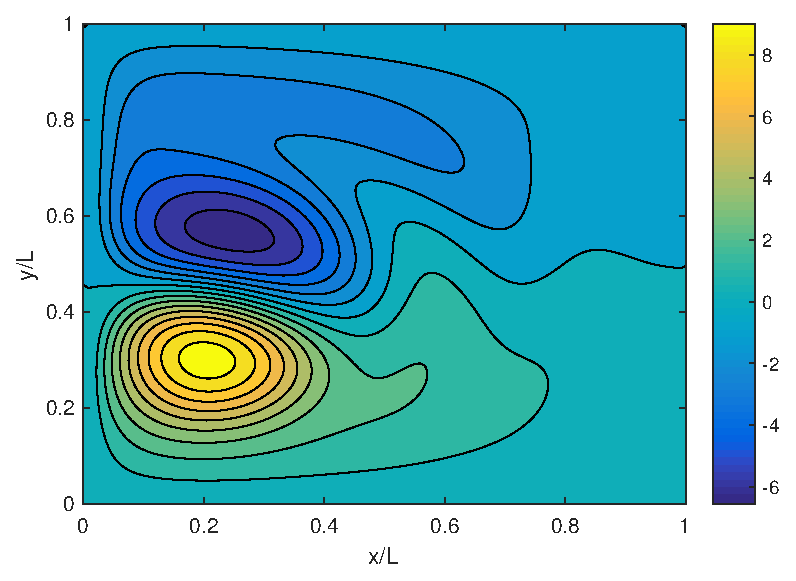
\includegraphics[width=\textwidth]{images/e_psi.eps}
        \caption{Streamfunction $\psi$ at $Re = 40$}
        \label{fig:question_e_psi}
    \end{subfigure}
    ~
    \begin{subfigure}[b]{0.6\textwidth}
        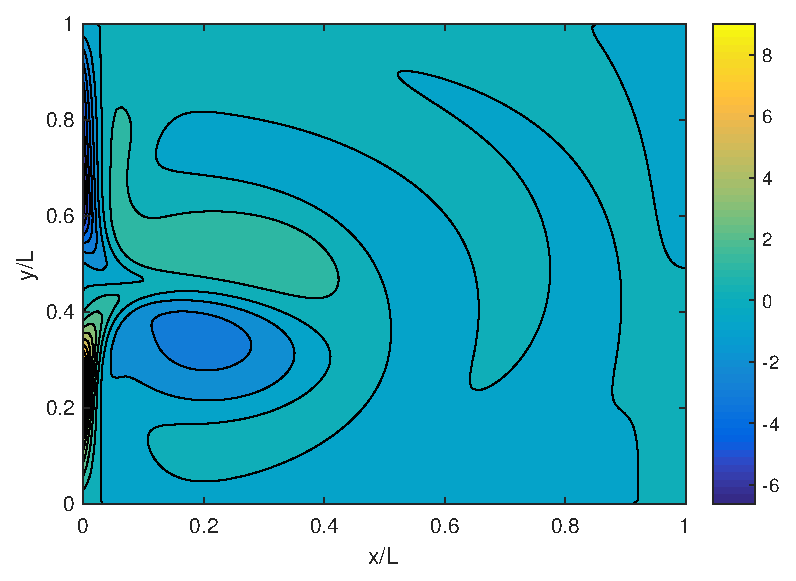
\includegraphics[width=\textwidth]{images/e_zeta.eps}
        \caption{$\zeta$ at $Re = 40$}
        \label{fig:question_e_zeta}
    \end{subfigure}
    }
\end{figure}

Now that we are on asymmetric branch of the pitchfork, we can easily get on its anti-symmetric counterpart by continuing backwards in $Re$ from $Re = 40$ to $Re_p$ and then all the way to $Re = 40$ again. This is done by setting $\Delta s = -1.$ We plot the solution in Figure~\ref{fig:question_e_lower}.

\begin{figure}[h]
    \centering
    \caption{Solutions on the lower branch of the pitchfork}\label{fig:question_e_lower}
    \centerline{
    \begin{subfigure}[b]{0.6\textwidth}
        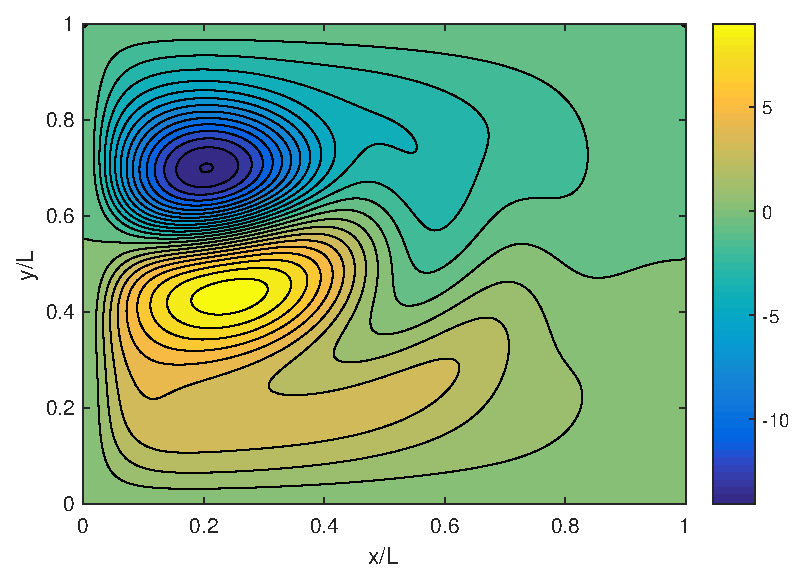
\includegraphics[width=\textwidth]{images/e_psi_lower.eps}
        \caption{Streamfunction $\psi$ at $Re = 40$}
        \label{fig:question_e_psi_lower}
    \end{subfigure}
    ~
    \begin{subfigure}[b]{0.6\textwidth}
        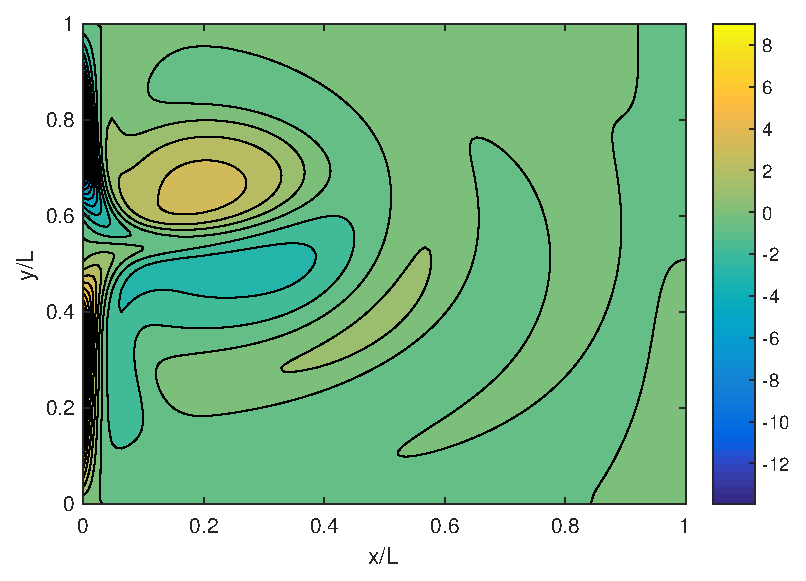
\includegraphics[width=\textwidth]{images/e_zeta_lower.eps}
        \caption{$\zeta$ at $Re = 40$}
        \label{fig:question_e_zeta_lower}
    \end{subfigure}
    }
\end{figure}